
\includegraphics[height=1.25cm]{images/pictograms/benchmark}

\includegraphics[height=1.25cm]{images/pictograms/FEM}

%%%%%%%%%%%%%%%%%%%%%%%%%%%%%%%%%%%%%%%%%%%%%%%%%%%%%%%%%%%%%%%%%%%%%%%%%%%%%%%%%%%%%%%%%%%%%%%%%%%

%\lstinputlisting[language=bash,basicstyle=\small]{python_codes/fieldstone_12/keywords.ascii}

\begin{center}
\inpython ~
{\small Code: \url{https://github.com/cedrict/fieldstone/tree/master/python_codes/fieldstone_12}}
\end{center}

\par\noindent\rule{\textwidth}{0.4pt}

Last revision: August 30th, 2025.

\par\noindent\rule{\textwidth}{0.4pt}

%%%%%%%%%%%%%%%%%%%%%%%%%%%%%%%%%%%%%%%%%%%%%%%%%%%%%%%%%%%%%%%%%%%%%%%%%%%%%%%%%%%%%%%%%%%%%%%%%%%

We start from the analytical benchmark of Section \ref{MMM-mms1} and we use $Q_1 \times P_0$
elements with a penalty formulation. 
We have seen in \stone~\ref{f01} how to recover the elemental pressure as a postprocessing step. 
However, the discontinous nature of the pressure field (and the presence of a
parasitic checkerboard mode) can be problematic for many reasons 
(pressure enters the rheology, equation of state, plotting, ...). 
We then wish to project the elemental pressure onto the nodes of the mesh while at the same 
time filtering the checkerboard mode out. 

Terminology: in general, when a discontinuous elemental pressure is used in a stone, 
it is called $p$ while its projection onto the velocity nodes is called $q$. 
In this case we compute several nodal pressures as explained in Section~\ref{MMM-psmoothing}:

\begin{itemize}
%...........
\item $q_1$: smoothed pressure obtained with the  center-to-node approach (scheme 1).

\item $q_2$: the nodal pressure obtained by smoothing the elemental pressure using element areas (scheme 2).

\item $q_3$: the nodal pressure obtained by smoothing the elemental p using triangle areas (scheme 3).

\item $q_4$: smoothed pressure obtained with the center-to-node approach with inverse element area weighing.

\item $q_5$: is not computed because same as 6.

\item $q_6$: consistent pressure recovery through FE (scheme 5 \& 6)

\item $q_7$: consistent pressure recovery with lumped mass matrix. 

\item $q_8$: bilinear interpolation. 

\end{itemize}

Since the D\& H setup showcases Dirichlet boundary conditions on all four sides, 
there is a pressure nullspace and it is removed 
by normalizing the pressure that $\int_\Omega p\; dV =0 $.

\begin{remark}
Nodes on edges and corners may need special treatment as documented in Sani et al \cite{sagl81a} or
Lee et al (1979) \cite{legs79} which is not done here.  
Nodes on the boundary showcase the largest errors. Maybe then use CBF instead for these?
\end{remark}

\begin{remark}
Lee et al (1979) \cite{legs79} discuss two different ways to compute the lumped mass matrix. 
\end{remark}

\begin{remark}
In the {\tt code\_simplefem\_consistent\_press} folder there is a fortran90 
version of the consistent recovery algorithm.
\end{remark}

There is much more work to be done on this topic/stone! Look at cost vs accuracy!

%------------------------------------------------------------------------
\subsection*{A (new) checkerboard filter?}

I have created a simple checkerboard filter. Let $\phi=\pm 1$ denote this field.
The filter is applied as follows:
\[
p_{filtered} = p - \left( \frac{1}{|\Omega|} \iint_\Omega p \phi dV \right) \phi
\]
It is in fact a projection. If $p=\alpha \phi$  where $\alpha$ is a scalar, then 
it is trivial to show that $p_{filtered} =0$:
\begin{eqnarray}
p_{filtered} 
&=& p - \left( \frac{1}{|\Omega|} \iint_\Omega p \phi dV \right) \phi \nn\\
&=& \alpha \phi - \left( \frac{1}{|\Omega|} \iint_\Omega \alpha \phi \phi dV \right) \phi \nn\\
&=& \alpha \phi - \left( \frac{1}{|\Omega|} \alpha \sum_e \iint_{\Omega_e} \phi^2 dV \right) \phi \nn\\
&=& \alpha \phi - \left( \frac{1}{|\Omega|} \alpha \sum_e \iint_{\Omega_e} 1 dV \right) \phi \nn\\
&=& \alpha \phi - \left( \frac{1}{|\Omega|} \alpha \sum_e |{\Omega_e}| \right) \phi \nn\\
&=& \alpha \phi - \left( \frac{1}{|\Omega|} \alpha |\Omega| \right) \phi \nn\\
&=& \alpha \phi - \alpha\phi \nn\\
&=& 0 
\end{eqnarray}
since on an element $\phi^2=1$. Here $|\Omega_e|$ is the volume of element $e$ and $|\Omega|$ is the 
volume of the whole domain.
This means that if the pressure field is 100\% made of a checkerboard field then the 
filter completely removes it.

Likewise, if $p=p_0=constant$ then 
\begin{eqnarray}
p_{filtered} 
&=& p_0 - \left( \frac{1}{|\Omega|} \iint_\Omega p_0 \phi dV \right) \phi \nn\\
&=& p_0 - \left( \frac{1}{|\Omega|} p_0 \iint_\Omega  \phi dV \right) \phi \nn\\ 
&=& p_0 - \left( \frac{1}{|\Omega|} p_0 \sum_e \iint_{\Omega_e}  \phi dV \right) \phi \nn
\end{eqnarray}
If there are as many $\phi=+1$ and $\phi=-1$ elements (i.e. the number of elements in 
each direction is even?) *and* the total volume of the '+' elements is equal 
to the total volume of the '-' elements then the integral above is zero and 
we obtain $p_{filtered}=p_0$.

What about the case where the mesh does not consist of equal size elements ?
\todo[inline]{I need to check but paper by Gang Lu states that then modes don't appear. }

In order to remove the explicit dependency on the areas of elements, 
the filter above can be reformulated as follows\footnote{if elements are 
equal size rectangles this formulation is identical to the one with integrals.}
\[
\boxed{
p_{filtered} = p - \left( \frac{1}{nel} \sum_e  \phi_e p_e \right) \phi
}
\]
Let us assume that the pressure field is linear and that a checkerboard mode 
of amplitude $\alpha$ is present on top of the real signal:
\[
p^h(x,y)=ax+by+c + \alpha \phi(x,y)
\]
We start with ($x_e,y_e$ stand for the coordinates of the element centers)
\begin{eqnarray}
&&\frac{1}{nel} \sum_e^{nel} p(x,_e,y_e) \phi(x_e,y_e) \nn\\
&=& \frac{1}{nel} \sum_e^{nel} \left[ ax_e+by_e+c + \alpha \phi(x_e,y_e)  \right] \phi(x_e,y_e) \nn\\
&=& \frac{1}{nel} \sum_e^{nel}  a x_e \phi(x_e,y_e) 
+ \frac{1}{nel} \sum_e^{nel} by_e  \phi(x_e,y_e) 
+ \frac{1}{nel} \sum_e^{nel} c  \phi(x_e,y_e) 
+ \frac{1}{nel} \sum_e^{nel} \alpha \phi(x_e,y_e)   \phi(x_e,y_e) \nn\\
&=& \frac{1}{nel} a \sum_e^{nel}   x_e \phi(x_e,y_e) 
+ \frac{1}{nel} b\sum_e^{nel} y_e  \phi(x_e,y_e) 
+ \underbrace{\frac{1}{nel} c\sum_e^{nel}   \phi(x_e,y_e) }_{=0}
+ \frac{1}{nel} \alpha \sum_e^{nel}  \underbrace{\phi(x_e,y_e)^2}_{=1} 
%&=& \frac{1}{nel} a \sum_e   x_e \phi(x_e,y_e) 
%+ \frac{1}{nel} b\sum_e y_e  \phi(x_e,y_e) 
%+ \frac{1}{nel} \alpha \underbrace{\sum_e  1}_{nel}
\end{eqnarray}
The third term is zero because of the even number of elements. 
The fourth one is simply equal to $\alpha$.
For the 1st and 2nd terms we rewrite the sum over elements as a double sum over the rows and 
columns of elements (assuming this a 2d problem for simplicity):
\[
\sum_e^{nel} = \sum_i^{nely} \sum_j^{nelx}
\]
where $i$ denotes a column and $j$ a row. Then 
\begin{eqnarray}
\frac{1}{nel} a \sum_e   x_e \phi(x_e,y_e)  + \frac{1}{nel} b\sum_e y_e  \phi(x_e,y_e) 
&=&\frac{1}{nel} a \sum_i\sum_j   x_i \phi(x_i,y_j)  + \frac{1}{nel} b \sum_i\sum_j y_j  \phi(x_i,y_j) \nn\\
&=&\frac{1}{nel} a \sum_i   x_i  \underbrace{\sum_j\phi(x_i,y_j)}_{=0}  
+ \frac{1}{nel} b \sum_j y_j  \underbrace{\sum_i\phi(x_i,y_j) }_{=0}\nn
\end{eqnarray}
Both these sums are zero because on one row or one column the sum of the $\phi$ function is zero. 
In the end we find
\begin{eqnarray}
\frac{1}{nel} \sum_e^{nel} p(x,_e,y_e) \phi(x_e,y_e)  = \alpha 
\end{eqnarray}
so that 
\begin{eqnarray}
p_{filtered} 
&=& p - \left( \frac{1}{nel} \sum_e^{nel} p(x,_e,y_e) \phi(x_e,y_e) \right)  \phi(x,y) \nn\\
&=& ax+by+c + \alpha \phi(x,y) - \alpha  \phi(x,y) \nn\\
&=& ax+by+c 
\end{eqnarray}
so that the filter was successful to remove a checkerboard pattern from a linear pressure field.


\begin{remark}
This idea is probably to be found in the relevant publications of Section~\ref{MMM-psmoothing}
in some form or shape? 
\end{remark}

\newpage
%---------------------------------------------------------------------------------
\subsection*{D\&H: Regular mesh made of square elements}

We compute the error convergence for $p$, $q_i$ $(i=1,...8)$:
\begin{center}
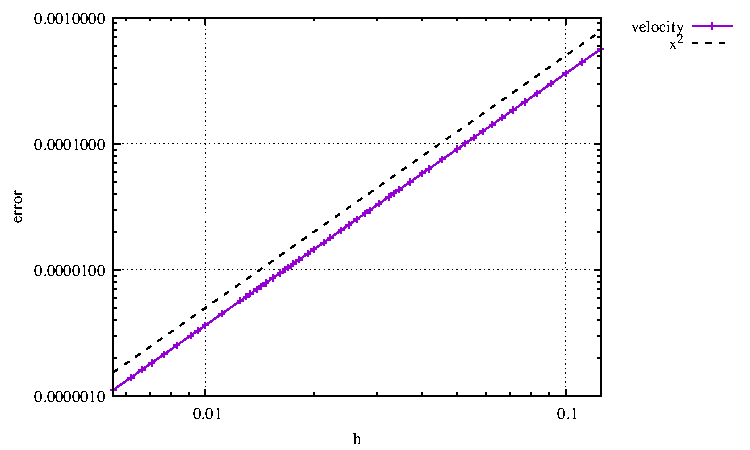
\includegraphics[width=8cm]{python_codes/fieldstone_12/results/reg/errorsV}
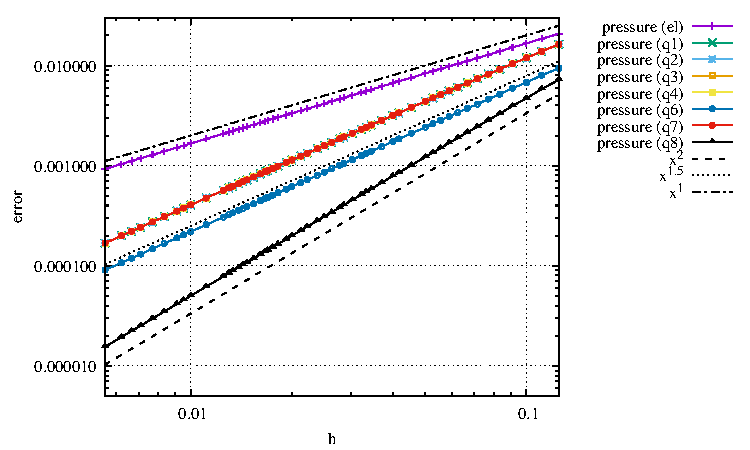
\includegraphics[width=8cm]{python_codes/fieldstone_12/results/reg/errorsP}
\end{center}
The elemental pressure error converges like $h^1$, $q_{1-7}$ converge like $h^{1.5}$ and 
$q^8$ converges like $h^2$.

\begin{center}
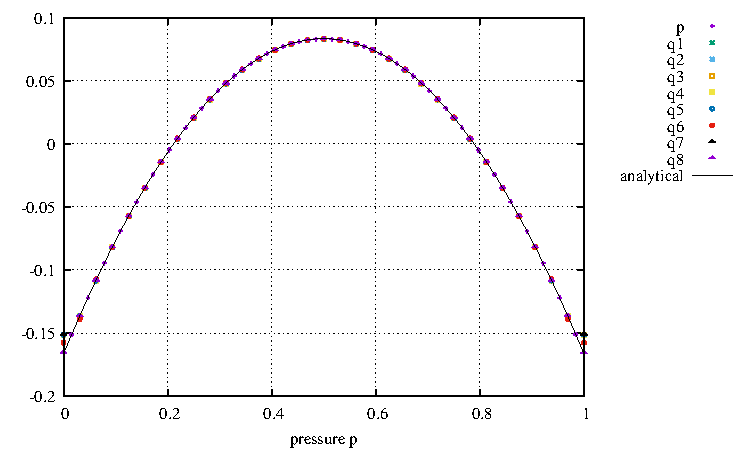
\includegraphics[width=8cm]{python_codes/fieldstone_12/results/reg/pressure}
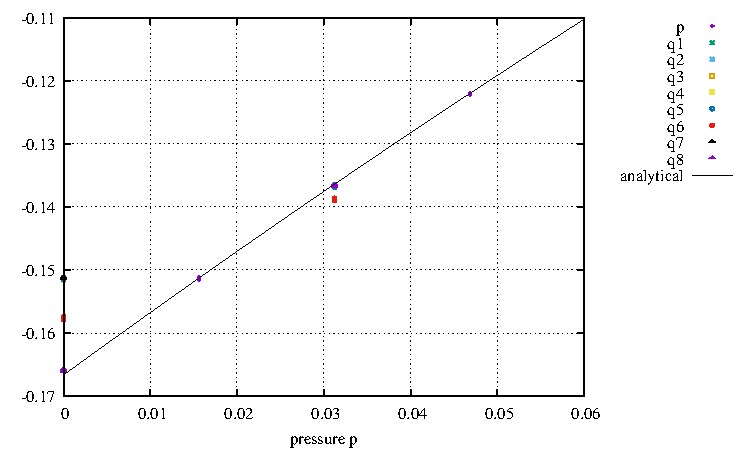
\includegraphics[width=8cm]{python_codes/fieldstone_12/results/reg/pressure_left}\\
{\captionfont fields $p$ and $q_{1-8}$ as a function of $x$. Right panel 
is a zoom around $x=0$}
\end{center}


\begin{center}
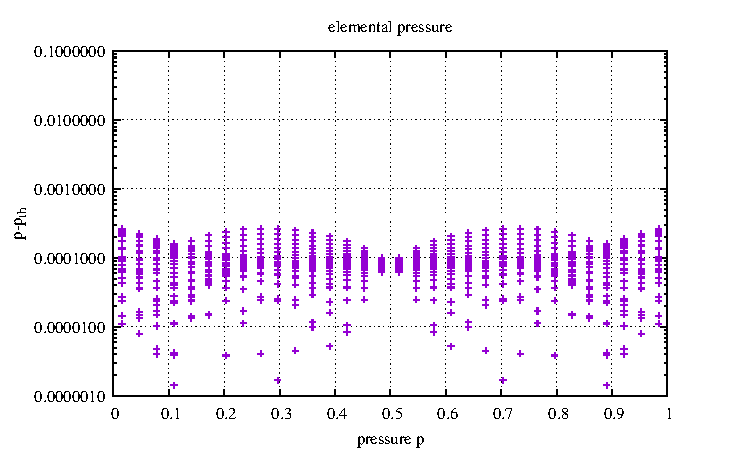
\includegraphics[width=4cm]{python_codes/fieldstone_12/results/reg/p_error}
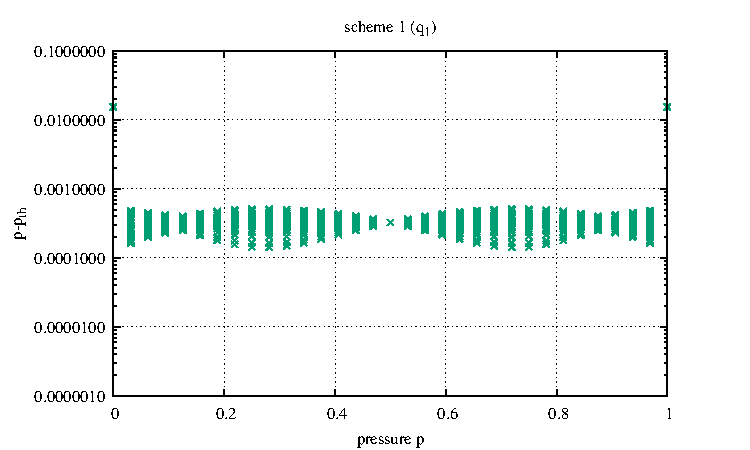
\includegraphics[width=4cm]{python_codes/fieldstone_12/results/reg/q1_error}
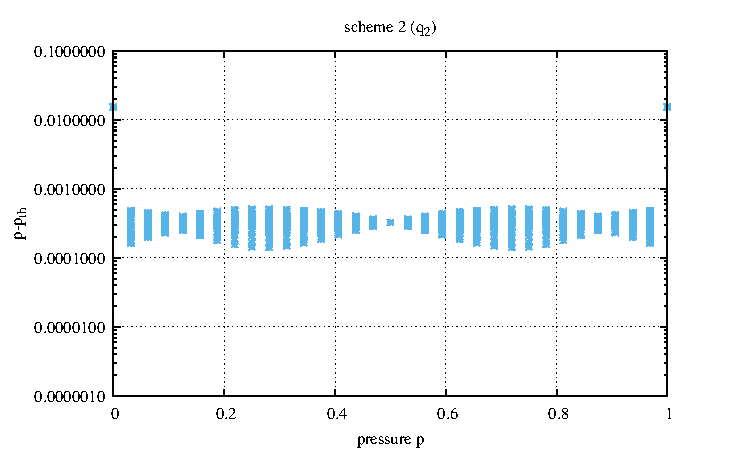
\includegraphics[width=4cm]{python_codes/fieldstone_12/results/reg/q2_error}
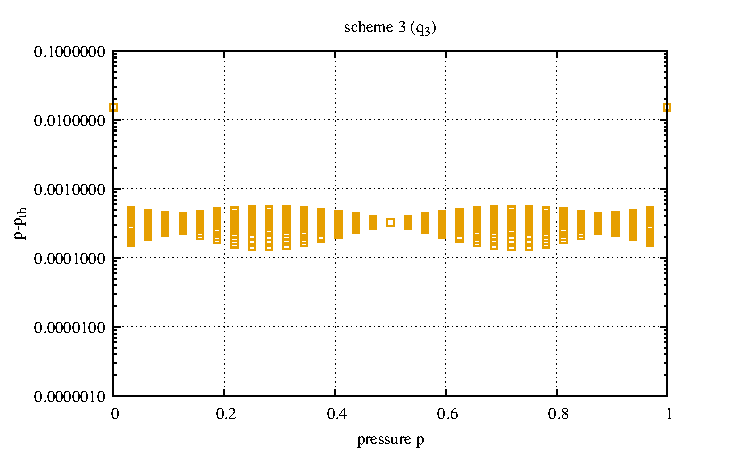
\includegraphics[width=4cm]{python_codes/fieldstone_12/results/reg/q3_error}\\
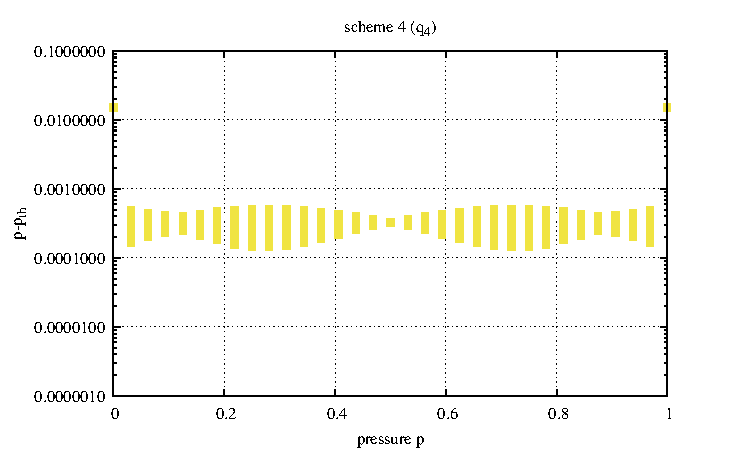
\includegraphics[width=4cm]{python_codes/fieldstone_12/results/reg/q4_error}
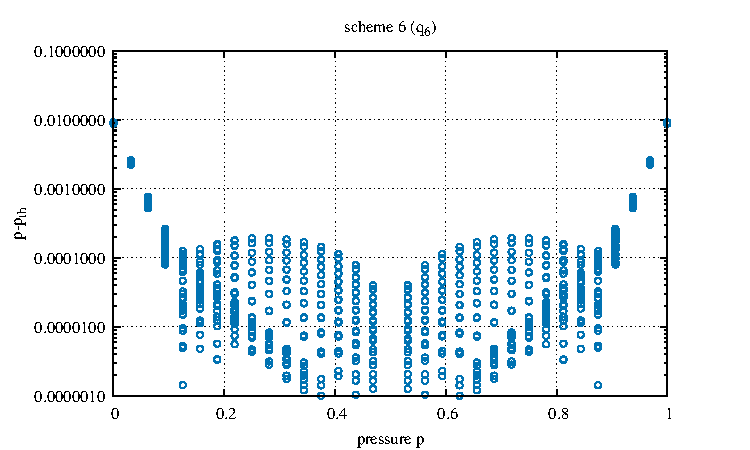
\includegraphics[width=4cm]{python_codes/fieldstone_12/results/reg/q6_error}
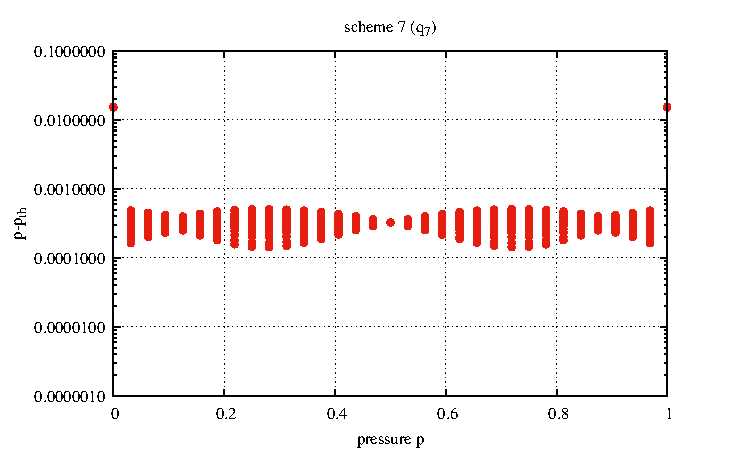
\includegraphics[width=4cm]{python_codes/fieldstone_12/results/reg/q7_error}
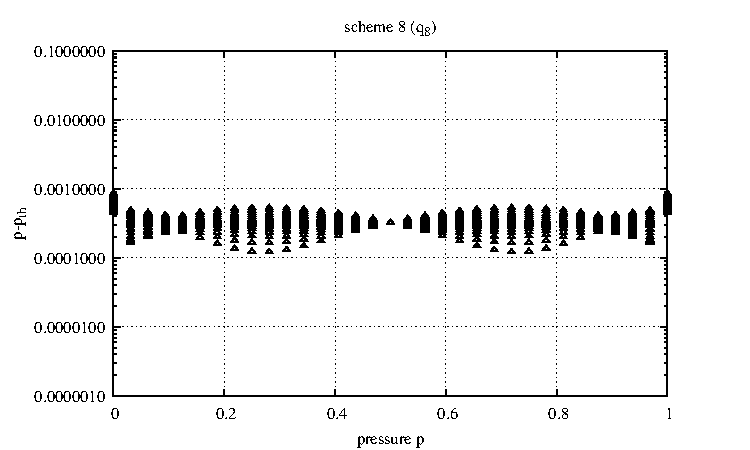
\includegraphics[width=4cm]{python_codes/fieldstone_12/results/reg/q8_error}\\
{\captionfont 
Absolute errore with regards to the analytical solution. All on $32\times 32$ mesh.}
\end{center}

\newpage
It is worth noticing that the checkerboard is (visually) not present:
\begin{center}
\includegraphics[width=5.6cm]{python_codes/fieldstone_12/results/reg/p32}
\includegraphics[width=5.6cm]{python_codes/fieldstone_12/results/reg/p48}
\includegraphics[width=5.6cm]{python_codes/fieldstone_12/results/reg/p64}\\
{\captionfont Elemental pressure field for 32x32, 48x48 and 64x64 resolutions.}
\end{center}
%This means that the algorithms above fulfill an interpolation function, but not a smoothing one.

Looking at the min/max/avg of the elemental pressure field 
with and without filter:
\begin{center}
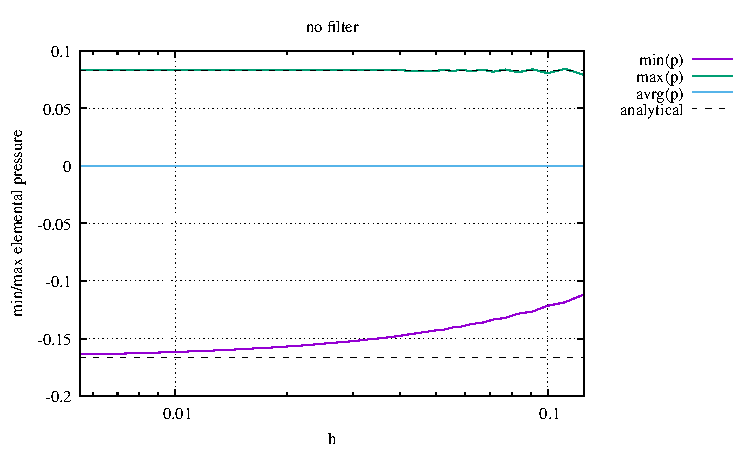
\includegraphics[width=7cm]{python_codes/fieldstone_12/results/reg/rawp_nofilter.pdf}
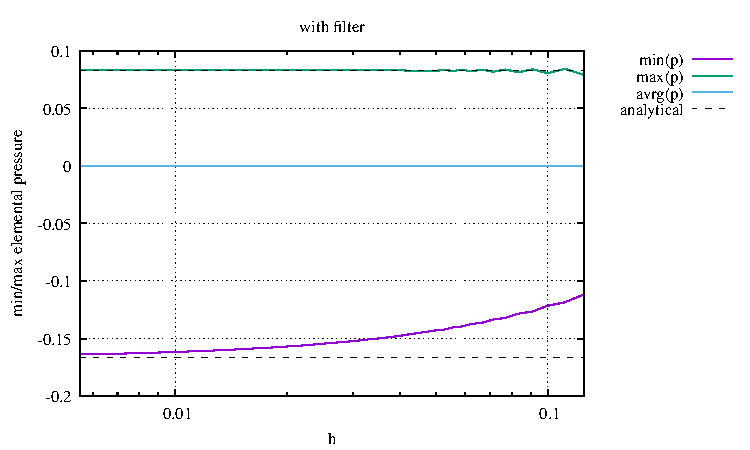
\includegraphics[width=7cm]{python_codes/fieldstone_12/results/reg/rawp_filter.pdf}\\
{\captionfont min/max/avrg elemental pressure as a function of element size.}
\end{center}
Unsurprisingly in this case the filter does not do much. 
We can verify this by looking at the elemental pressure error convergence:

\begin{center}
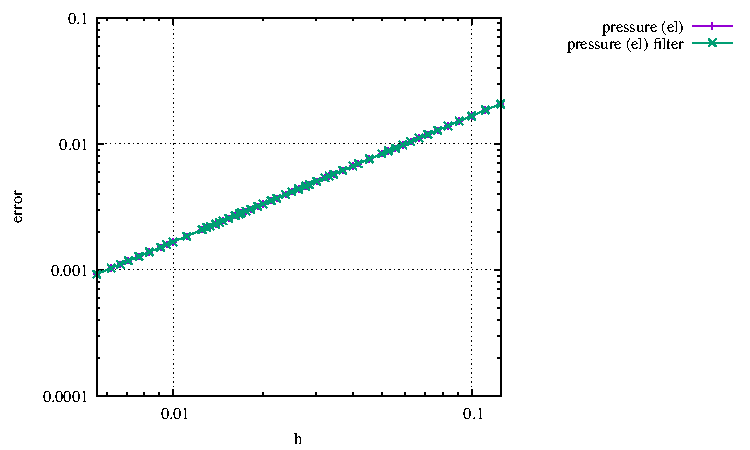
\includegraphics[width=8cm]{python_codes/fieldstone_12/results/reg/errorsP_both.pdf}
\end{center}
In this case the filter does virtually nothing.


\newpage
%............................................
\subsection*{D\&H: Adding randomness to internal node positions} We now add a random value $\xi h$ to the 
location of all nodes which are not on the boundary where $h$=$L_x$/nelx and we set $\xi=20\%$.
In this case a $32\times 32$ mesh looks as follows:

\begin{center}
\includegraphics[width=8cm]{python_codes/fieldstone_12/results/rand/area_0p1}
\includegraphics[width=8cm]{python_codes/fieldstone_12/results/rand/area_0p2}\\
{\captionfont Mesh 32x32 elements. Left: $\xi=0.1$; Right: $\xi=0.2$}
\end{center}

We repeat the same exercise as before on such a mesh and look at the errors

\begin{center}
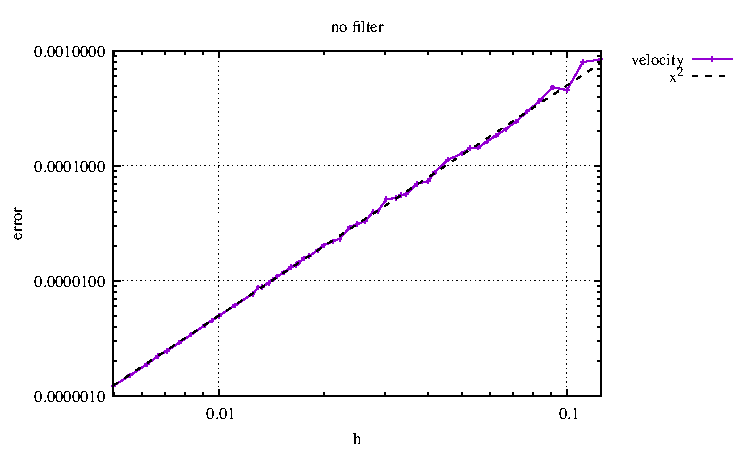
\includegraphics[width=8cm]{python_codes/fieldstone_12/results/rand/errorsV_nofilter}
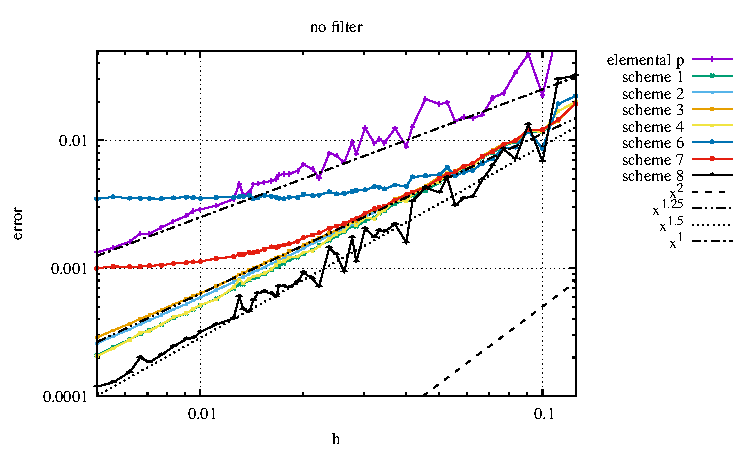
\includegraphics[width=8cm]{python_codes/fieldstone_12/results/rand/errorsP_nofilter}\\
{\captionfont Velocity and pressure errors for $\xi=0.2$. No filter.}
\end{center} 


\begin{center}
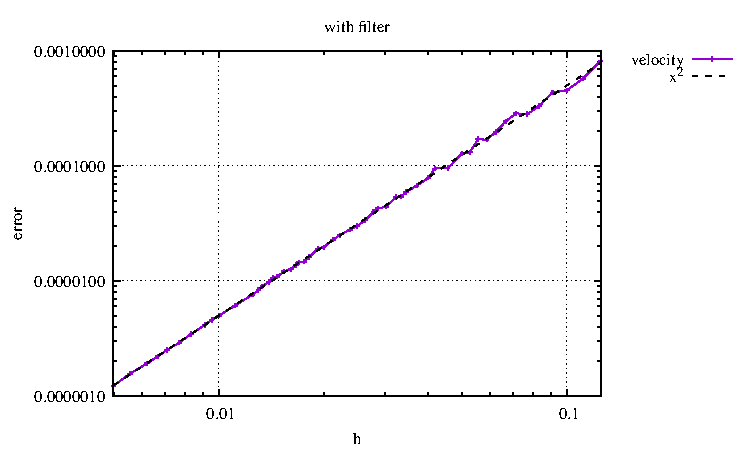
\includegraphics[width=8cm]{python_codes/fieldstone_12/results/rand/errorsV_filter}
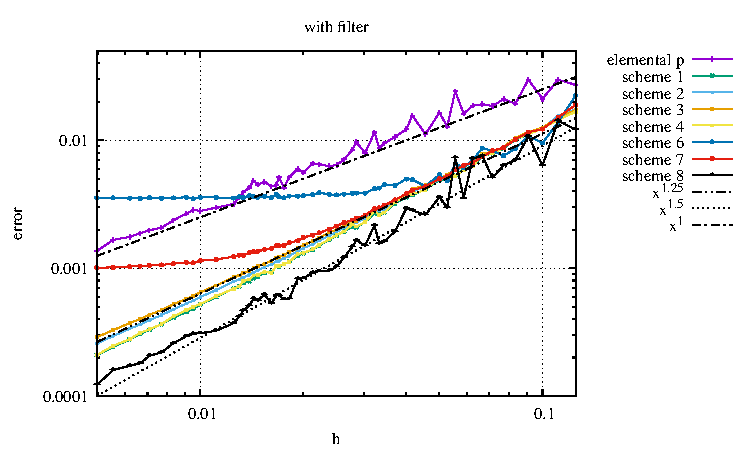
\includegraphics[width=8cm]{python_codes/fieldstone_12/results/rand/errorsP_filter}\\
{\captionfont Velocity and pressure errors for $\xi=0.2$. With filter.} 
\end{center}

It is easy to see the drastic effect that the filter has on the min/max of the elemental pressure:
\begin{center}
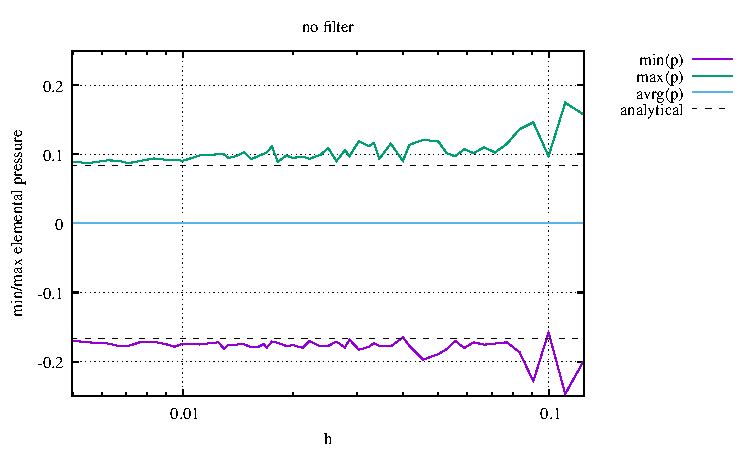
\includegraphics[width=7cm]{python_codes/fieldstone_12/results/rand/rawp_nofilter}
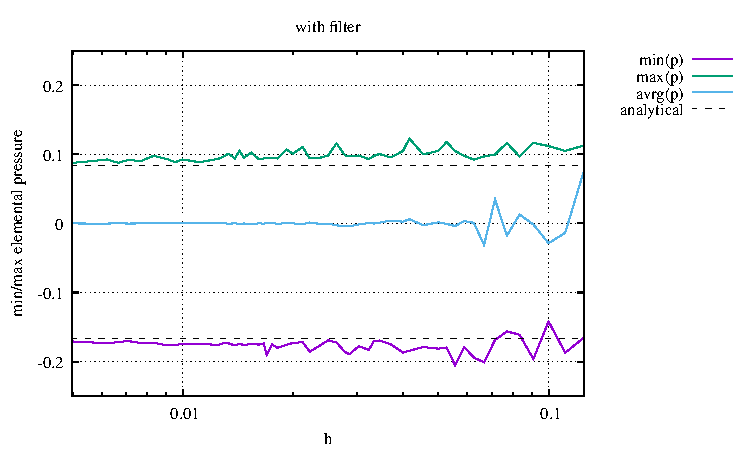
\includegraphics[width=7cm]{python_codes/fieldstone_12/results/rand/rawp_filter}\\
{\captionfont Min/max value of elemental pressure field: Left: no filter, right: with filter}
\end{center}

Rather surprisingly we find that $q_1$ still proves to be the most accurate of all pressures and it converges
with $h^{1.5}$(?) as before. Because checkerboard modes are triggered the convergence of the elemental 
pressure is more chaotic but on average linear. 
The $q_6$ and $q_7$ fields seem to unexpectedly stop converging above a given resolution, which 
probably comes from the lack of adequate treatment of sides and corners.
All others converge with $h^{1.5}$ and $q_4$ seems a bit more chaotic than the others.
Scheme 8 seems to be the best here again but with an erratic convergence about $h^{1.5}$

\begin{center}
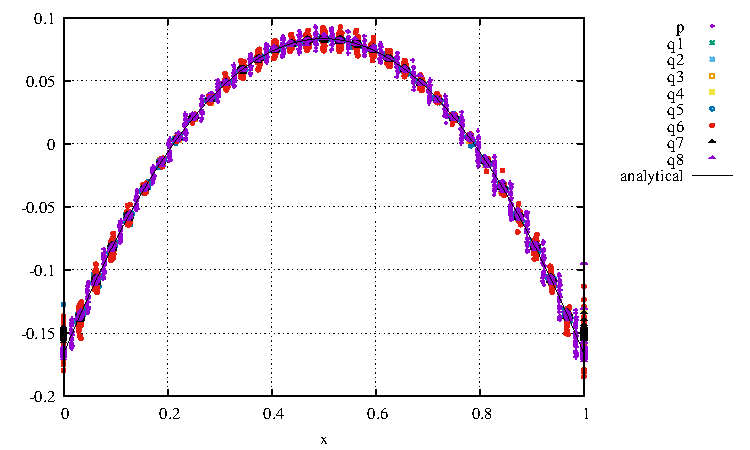
\includegraphics[width=5cm]{python_codes/fieldstone_12/results/rand/pressure}
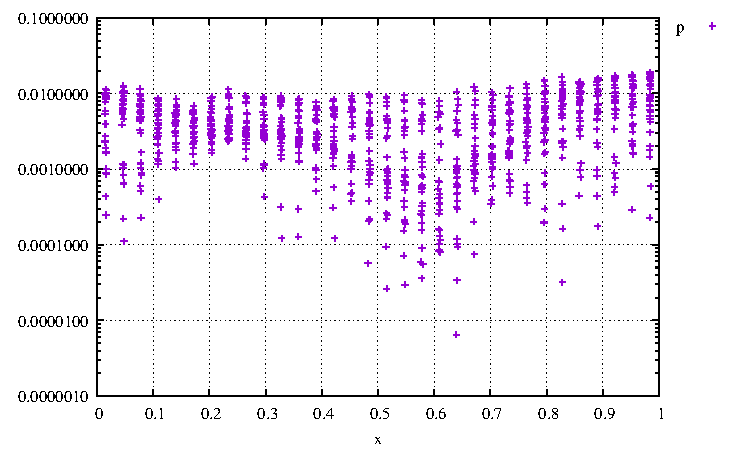
\includegraphics[width=5cm]{python_codes/fieldstone_12/results/rand/p_error}
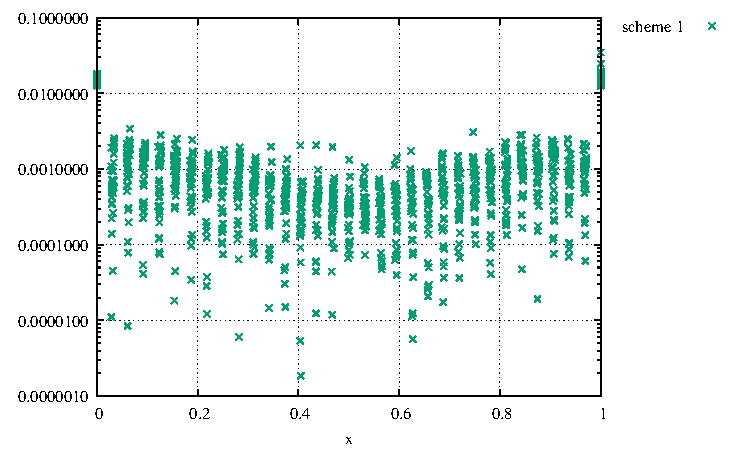
\includegraphics[width=5cm]{python_codes/fieldstone_12/results/rand/q1_error}\\
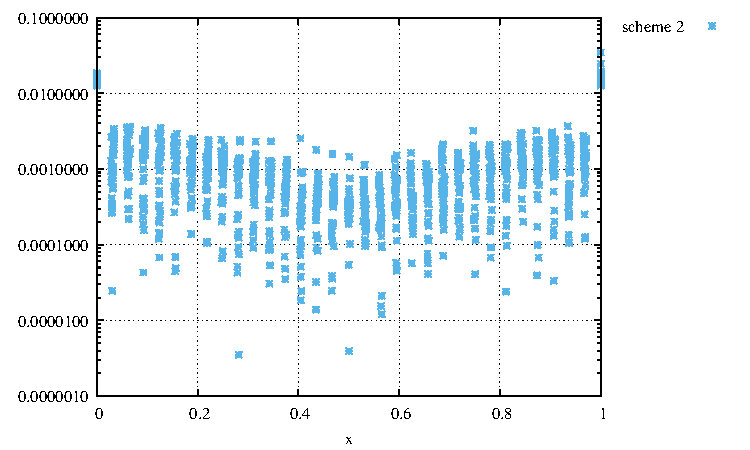
\includegraphics[width=5cm]{python_codes/fieldstone_12/results/rand/q2_error}
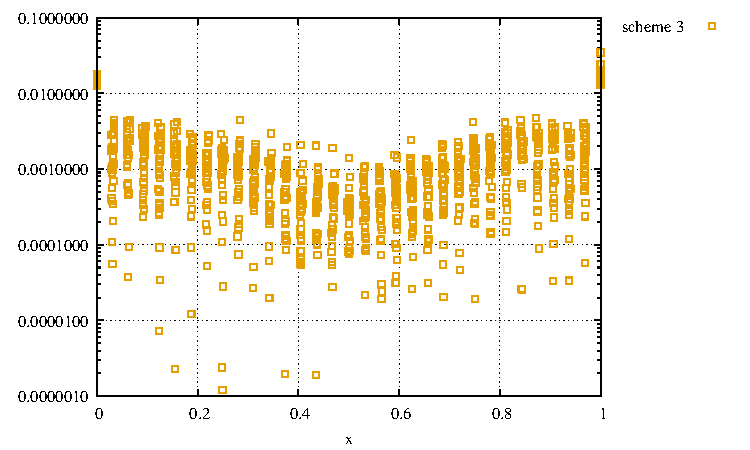
\includegraphics[width=5cm]{python_codes/fieldstone_12/results/rand/q3_error}
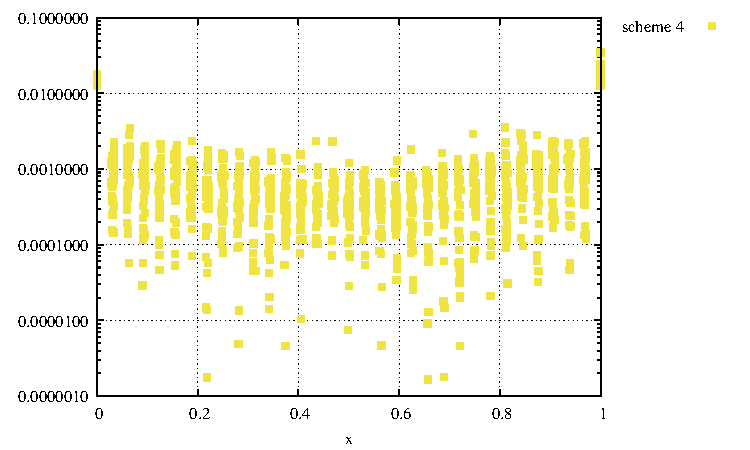
\includegraphics[width=5cm]{python_codes/fieldstone_12/results/rand/q4_error}\\
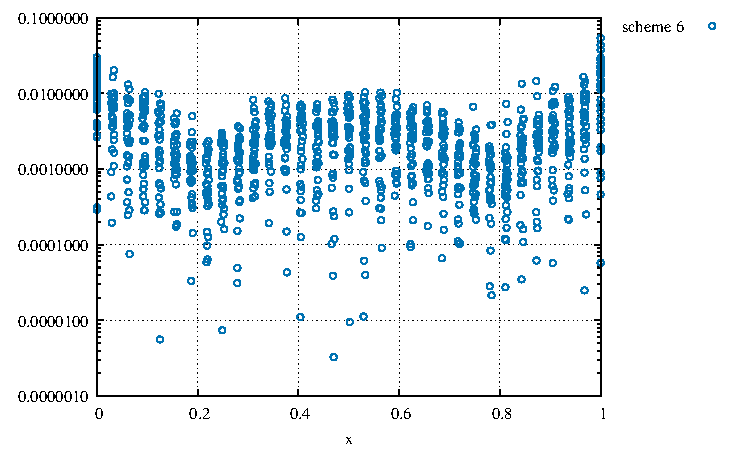
\includegraphics[width=5cm]{python_codes/fieldstone_12/results/rand/q6_error}
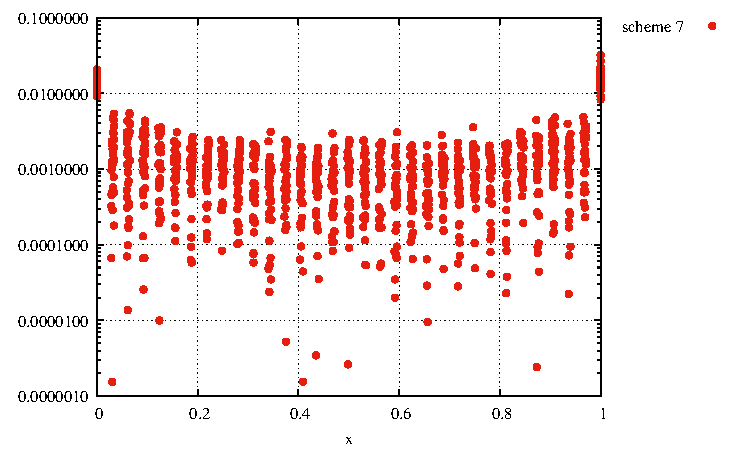
\includegraphics[width=5cm]{python_codes/fieldstone_12/results/rand/q7_error}
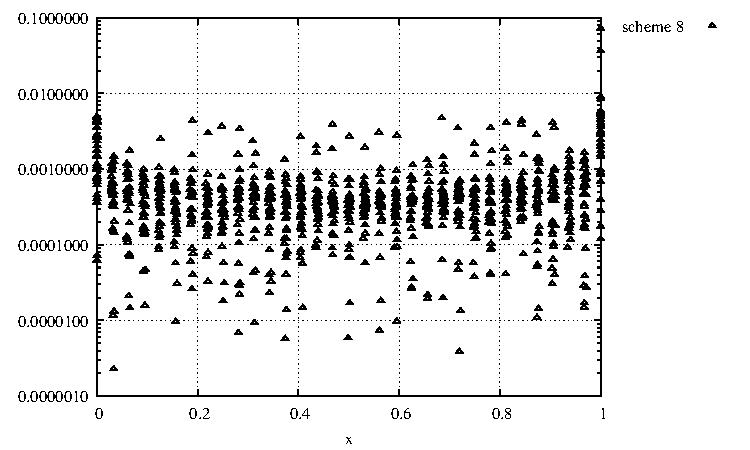
\includegraphics[width=5cm]{python_codes/fieldstone_12/results/rand/q8_error}\\
{\captionfont all obtained in 32x32 mesh}
\end{center}

\begin{center}
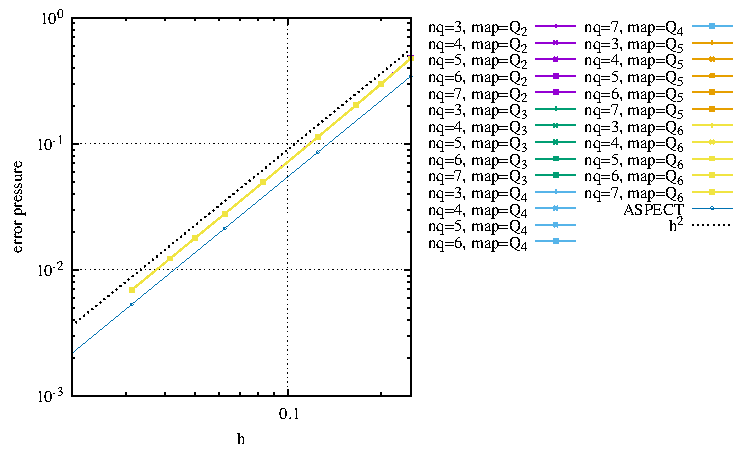
\includegraphics[width=5cm]{python_codes/fieldstone_12/results/rand/errp}
\includegraphics[width=5cm]{python_codes/fieldstone_12/results/rand/errq1}
\includegraphics[width=5cm]{python_codes/fieldstone_12/results/rand/errq2}\\
\includegraphics[width=5cm]{python_codes/fieldstone_12/results/rand/errq3}
\includegraphics[width=5cm]{python_codes/fieldstone_12/results/rand/errq4}
\includegraphics[width=5cm]{python_codes/fieldstone_12/results/rand/errq6}\\
\includegraphics[width=5cm]{python_codes/fieldstone_12/results/rand/errq7}
\includegraphics[width=5cm]{python_codes/fieldstone_12/results/rand/errq8}\\
{\captionfont Pressure error for the elemental and nodal pressure fields. Note 
the presence of a spatially varying checkboard pattern in the elemental pressure field.
Obtained on 32x32 mesh.}
\end{center}


\newpage
%............................................
\subsection*{Lid driven cavity}

This experiment is not a benchmark since no analytical solution is available.
The domain is a unit square and the mesh consists of square elements. 
No slip boundary conditions are prescribed 
on left, right and bottom boundary. Unit velocity is prescribed on the top, 
including both top corners, in order to generate a velocity/pressure discontinuity  
which triggers the checkerboard. This is rather succesful (no filter is applied yet):

\begin{center}
\includegraphics[width=7cm]{python_codes/fieldstone_12/results/ldc32/vel}
\includegraphics[width=7cm]{python_codes/fieldstone_12/results/ldc33/vel}\\
\includegraphics[width=7cm]{python_codes/fieldstone_12/results/ldc32/p}
\includegraphics[width=7cm]{python_codes/fieldstone_12/results/ldc33/p}\\
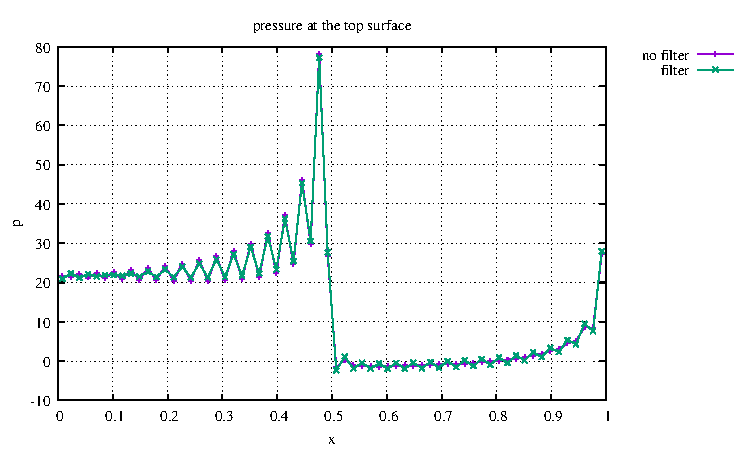
\includegraphics[width=7cm]{python_codes/fieldstone_12/results/ldc32/p_top}
\includegraphics[width=7cm]{python_codes/fieldstone_12/results/ldc33/p_top}\\
{\captionfont Left: 32x32, Right: 33x33. Last row is pressures at the top of the domain.}
\end{center}

We recover the well known fact that even number of elements are more prone to 
checkerboard of high amplitude, but odd numbers do not preclude their presence.
The conclusion is unescapable: there is no nodal pressure field which does not 
showcase some positive/negative oscillations.

It is easy to see the drastic effect that the filter has on the min/max of the elemental pressure:

\begin{center}
\includegraphics[width=8cm]{python_codes/fieldstone_12/results/ldc/prms_even_nofilter}
\includegraphics[width=8cm]{python_codes/fieldstone_12/results/ldc/prms_odd_nofilter}\\
\includegraphics[width=8cm]{python_codes/fieldstone_12/results/ldc/prms_even_filter}
\includegraphics[width=8cm]{python_codes/fieldstone_12/results/ldc/prms_odd_filter}\\
{\captionfont root mean square pressure. Left: filter off; Right: filter on.
Notice the wildly different vertical scales between both figures.}
\end{center}

\begin{center}
\includegraphics[width=8cm]{python_codes/fieldstone_12/results/ldc/rawp_even_nofilter}
\includegraphics[width=8cm]{python_codes/fieldstone_12/results/ldc/rawp_odd_nofilter}\\
\includegraphics[width=8cm]{python_codes/fieldstone_12/results/ldc/rawp_even_filter}
\includegraphics[width=8cm]{python_codes/fieldstone_12/results/ldc/rawp_odd_filter}\\
{\captionfont min/max pressure. Left: filter off; Right: filter on. Notice the 
difference in scales for the $y$-axis. On the left we see that the amplitude of the 
checkerboard is unpredictable and varies across a few orders of magnitude.}
\end{center}

It is also worth remembering that this problem is somewhat ill-posed. 
The pressure should be infinite in the top corners

\todo[inline]{Run this with Q2 elements?}

%Only schemes 6 and 7 are unaffected by the filter since they 


\newpage
%............................................
\subsection*{Regularised Lid driven cavity}

See stone 4. The velocity on the top is given by $u(x)=x^2(1-x)^2$.
This has the advantage of removing the discontinuity at the corners and 
thereby yielding a problem which has a non-singular solution.
We see that the checkerboard mode is still present:

\begin{center}
\includegraphics[width=8cm]{python_codes/fieldstone_12/results/rldc/vel}
\includegraphics[width=8cm]{python_codes/fieldstone_12/results/rldc/p}\\
{\captionfont Resolution $64\times 64$.}
\end{center}

Again, there is no analytical solution. When the pressure errors are computed in the code
the results are actually root mean square pressures (if a zero analytical pressure 
is used). We see that these all converge to a single value.
We see that the filter has a drastic effect on the min/max 
of the elemental pressure (mind the $y$-axis range on these figures): 

\begin{center}
\includegraphics[width=7cm]{python_codes/fieldstone_12/results/rldc/prms_even_nofilter}
\includegraphics[width=7cm]{python_codes/fieldstone_12/results/rldc/prms_odd_nofilter}\\
\includegraphics[width=7cm]{python_codes/fieldstone_12/results/rldc/prms_even_filter}
\includegraphics[width=7cm]{python_codes/fieldstone_12/results/rldc/prms_odd_filter}\\
\end{center}

\begin{center}
\includegraphics[width=7cm]{python_codes/fieldstone_12/results/rldc/rawp_even_nofilter}
\includegraphics[width=7cm]{python_codes/fieldstone_12/results/rldc/rawp_odd_nofilter}\\
\includegraphics[width=7cm]{python_codes/fieldstone_12/results/rldc/rawp_even_filter}
\includegraphics[width=7cm]{python_codes/fieldstone_12/results/rldc/rawp_odd_filter}\\
{\captionfont Left: filter off; Right: filter on}
\end{center}


\newpage
%-----------------------------------------------------------------------------
\subsection*{A punch like experiment}

The domain is still the unit square. The boundary conditions are given by
\begin{lstlisting}
or i in range(0,NV):
   if y[i]<eps:
      bc_fix[i*ndof]   = True ; bc_val[i*ndof]   = 0.
      bc_fix[i*ndof+1] = True ; bc_val[i*ndof+1] = 0.
   if y[i]>(Ly-eps) and x[i]<0.5:
      bc_fix[i*ndof]   = True ; bc_val[i*ndof]   = 0
      bc_fix[i*ndof+1] = True ; bc_val[i*ndof+1] = -1.
   if x[i]<eps:
      bc_fix[i*ndof]   = True ; bc_val[i*ndof]   = 0.
   if x[i]>(Lx-eps):
      bc_fix[i*ndof]   = True ; bc_val[i*ndof]   = 0.
      bc_fix[i*ndof+1] = True ; bc_val[i*ndof+1] = 0.
\end{lstlisting}
In other words, the velocity is $v=-1$ on the left half of the top boundary, 
free slip on the left, no slip on the bottom and right:
\begin{center}
\includegraphics[width=7cm]{python_codes/fieldstone_12/results/punch/vel}
\end{center}





\begin{center}
\includegraphics[width=7cm]{python_codes/fieldstone_12/results/punch/prms_even_nofilter}
\includegraphics[width=7cm]{python_codes/fieldstone_12/results/punch/prms_odd_nofilter}\\
\includegraphics[width=7cm]{python_codes/fieldstone_12/results/punch/prms_even_filter}
\includegraphics[width=7cm]{python_codes/fieldstone_12/results/punch/prms_odd_filter}\\
\end{center}

\begin{center}
\includegraphics[width=7cm]{python_codes/fieldstone_12/results/punch/rawp_even_nofilter}
\includegraphics[width=7cm]{python_codes/fieldstone_12/results/punch/rawp_odd_nofilter}\\
\includegraphics[width=7cm]{python_codes/fieldstone_12/results/punch/rawp_even_filter}
\includegraphics[width=7cm]{python_codes/fieldstone_12/results/punch/rawp_odd_filter}\\
{\captionfont Left: filter off; Right: filter on}
\end{center}

\begin{center}
\includegraphics[width=8cm]{python_codes/fieldstone_12/results/punch/p_top.pdf}
\includegraphics[width=8cm]{python_codes/fieldstone_12/results/punch/p_top_all.pdf}\\
{\captionfont Left: filter vs no filter; Right: all $q$ pressures no filter.}
\end{center}

\begin{center}
\includegraphics[width=10cm]{python_codes/fieldstone_12/results/punch/pressures}\\
{\captionfont Left: no filter; Right: with filter.}
\end{center}

This is the nail in the coffin for the filter I propose.
Contrarily to the previous experiments, the checkerboard mode 
amplitude is not constant in space so that removing $\alpha \phi$
from the raw pressure does not remove the checkerboard at all. 










